\documentclass[sigconf]{acmart}

\input{format/final}

\begin{document}
  \title{Comparing Predictive Models of Pain Reliever Misuse and Abuse}
  \author{Sean M. Shiverick}
  \affiliation{\institution{Indiana University-Bloomington}
  }
\renewcommand{\shortauthors}{S.M. Shiverick}

%%%%%%%%%%%%%%%%%%%%%%%%%%%%%%%%%%%%%%%%%%%%%%%%%%%%%%%%%%%%%%%%%%%%%%%%%%%%%%%%

\begin{abstract}

The misuse and abuse of prescription opioids (MUPO) has become a major 
health crisis resulting in increased overdose deaths \cite{nida18}. Predictive 
modeling can identify factors related to MUPO and  predict individuals at risk 
for opioid addiction. The present study compares ten classification models 
using four performance metrics: accuracy, sensitivity (recall), precision, and 
$f_1$-score. Three years of data from the National Survey on Drug Use and 
Health (2015-2017) was combined to create a sample consisted of N = 170317
observations. Twenty-six percent of respondents reported using prescription
opioid medications in the past year, 11\% of respondents reported pain 
reliever misused or abuse, and 2\% reported using heroin. With unbalanced 
classes in the data, the $f_1$-score was used as the performance metric 
rather than accuracy. The classifier models were fit to the training set with 
fifteen features, including demographic variables, past medication use, and 
illicit drug use. The binary target variable was pain reliever misuse and abuse. 
Model performance was evaluated on the testing set. Logistic regression, 
decision trees, and random forests had the highest $f_1$-scores. Neural networks 
(MLP) and support vector classifier both had high accuracy, but low $f_1$-scores. Advantages and limitations of the classification models are discussed. 
\footnote{This project was done in partial fulfillment of requirements 
for the M.S. in Data Science from the School of Informatics and Computing at 
IU-Bloomington completed in May, 2018. Address correspondence to \textit{smshiver@iu.edu}}

\end{abstract}
\keywords{Predictive Modeling, Supervised Learning, Classification Models}
\maketitle

%%%%%%%%%%%%%%%%%%%%%%%%%%%%%%%%%%%%%%%%%%%%%%%%%%%%%%%%%%%%%%%%%%%%%%%%%%%%%%%%
\section{Introduction}

Over the past two decades the misuse and abuse of prescription opioids 
(MUPO) has become a major health crisis in the U.S. \cite{volkow14}. In 2015, 
an estimated 2 million Americans suffered a substance use disorder related 
to prescription opioid pain relievers such as oxycodone or hydrocodone 
\cite{nida18}. Opioid dependence and addiction are chronic health conditions. 
On average, more than 115 people die from an opioid overdose in the U.S. 
each day \cite{cdc18}, and the number of opioid-related overdose deaths has 
more than quadrupled from 1999 to 2016. Nonmedical use of prescription opioids 
is a significant risk factor for heroin use \cite{Rudd16}. Supply-based 
interventions to reduce the availability of prescription opioids have produced 
a shift to the use of heroin and synthetic opioids such as fentanyl 
\cite{jones15}. Four in five new heroin users started out misusing prescription 
painkillers \cite{jones13}. Because the dosage levels and potency of illicit 
or synthetic opioids are largely unknown, the risk of overdose death is greatly 
increased. The sharp rise in prescription overdose deaths (POD) and heroin 
overdose deaths (HOD) are correlated \cite{muhuri13, unick13}. Predictive 
modeling can be used to identify important features that contribute to the 
opioid misuse and abuse help predict individuals susceptible to opioid 
addiction. Data mining may provide insights to inform policy decisions for 
addressing the opioid crisis. This study compares the performance of several 
classification models to determine which approaches are best for
modeling pain reliever misuse and abuse. 

%%%%%%%%%%%%%%%%%%%%%%%%%%%%%%%%%%%%%%%%%%%%%%%%%%%%%%%%%%%%%%%%%%%%%%%%%%%%%%%%

\subsection{Predictive Modeling}

Predictive modeling, statistical learning, or machine learning describe a 
set of procedures and automated processes for extracting knowledge from data 
\cite{james13, kuhn13, muller17, raschka17}. The two main branches of 
predictive modeling are supervised learning and unsupervised learning. 
Supervised learning problems involve prediction about a specific target 
variable or outcome. If a dataset has no target outcome, unsupervised learning 
methods (e.g., clustering) can be used to discover underlying structure 
in unlabeled data. Supervised learning is used to predict a certain outcome 
from a given input, when examples of input/output pairs are available in the 
data (e.g., logistic regression) \cite{muller17}. A statistical learning model 
is constructed on a set of observations used to train the model set and then 
used to predict new observations. Two main approaches for supervised learning 
problems are regression and classification. When the target variable
to be predicted is continuous, or there is continuity between the outcome 
(e.g., home values), a regression model is used to test the set of features 
that predict the target variable. If the target is a class label, set of 
categorical or binary outcomes (e.g., spam or ham emails, benign or malignant 
cells), then classification can be used to predict which class or category 
label that new instances will be assigned to. This study uses a supervised 
learning approach to classify instances of pain reliever misuse and abuse
as a binary outcome. 

%%%%%%%%%%%%%%%%%%%%%%%%%%%%%%%%%%%%%%%%%%%%%%%%%%%%%%%%%%%%%%%%%%%%%%%%%%%%%%%%

In the era of ``big data'', large amounts of health information are being 
generated from electronic medical records (EMRs), clinical research data, to 
population-level health data \cite{herland14}. Although it can be difficult 
to obtain reliable information about opioid use based on self-reports, surveys 
provide data on a range of issues that people may be reluctant to disclose 
such as illicit drug use and mental health problems. The data for the present 
study was obtained from the National Survey on Drug Use and Health (NSDUH) 
which is a major source of information for the use of illicit drugs and mental 
health issues among the U.S. population aged 12 or older \cite{samhsa18}. 
The NSDUH is a comprehensive public survey that includes more than 2600 
variables on a diverse array of questions related to the use, misuse, and 
abuse of substances including alcohol, tobacco, prescription medications, and 
illicit drugs. In addition to typical demographic information, the survey
includes self-reported measures on items related to physical health, mental 
health (e.g., depression, anxiety, suicide), counseling, drug and alcohol 
treatment. Data from the NSDUH has been used for identifying groups at high 
risk for substance use, and the co-occurrence of substance use and mental 
health disorders. The target outcome for the study was any misuse or abuse 
of prescription pain relievers and the predictor variables of interest were 
demographic variables, medication usage, and use of illicit drugs. 

%%%%%%%%%%%%%%%%%%%%%%%%%%%%%%%%%%%%%%%%%%%%%%%%%%%%%%%%%%%%%%%%%%%%%%%%%%%%%%%%

\subsection{Classification Models}

\subsubsection{Linear Models}

As the statistician George Box stated, "All models are wrong, but some models 
are useful" \cite{box05}. There are advantages and limitations for selecting
any model. Logistic regression is one of the most reliable and interpretable 
models for classification. Logistic regression models the conditional 
distribution of probabilities for a binary response (e.g., $Pr(Y=k|X=x)$) 
as a combination of a set of predictor variables \cite{james13, raschka17}. 
The decision boundary for the logistic regression classifier is a linear 
function of the input; a binary classifier separates two classes using a line, 
plane, or hyperplane \cite{muller17}. Given that the probability values for 
the outcome range between 0 and 1, predictions can be made based on a default 
value. A default value of `Yes` could be predicted for any individual 
for whom the probability of pain reliever misuse and abuse is greater than 
fifty-percent, $Pr(PRLMISAB) > 0.5$. Logistic regression uses a maximum 
likelihood method to predict the coefficient estimates that correspond as 
closely as possible to the default state. In other words, the model will 
predict a number close to one for individuals who have misused or abused 
pain relievers and a number close to zero for individuals who have not. 
The distribution of conditional probabilities in the logit model has an 
S-shaped curve. The coefficient estimates are selected to maximize the 
likelihood function, and are interpreted as an indication of the log-odds 
change in the outcome variable that is associated with a one-unit increase 
in the predictor variable, holding the effects of other predictor variables 
constant. The intercept, $\beta_0$, is the log of the odds ratio when X 
is 0 \cite{gujarati09}. The logistic function is represented below, 
where X = ($X_1$...$X_p$) predictors: 

\begin{equation}
  \ ln\frac{P_i}{1-P_i} = \beta_0 + \beta_1X_1 + \beta_1X_2 +... \beta_p*X_p \
\end{equation}

\emph{Linear discriminant analysis} (LDA) is an alternative approach to 
estimating probabilities that models the distribution of predictors 
separately in each of the response classes and then uses the Bayes' theorem 
to `flip' these into estimates for $Pr(Y=k | X=x)$ \cite{james13}. The term 
linear in LDA refers to the the discriminant functions being linear functions 
of the predictors. For distributions assumed to be normal (i.e., multivariate 
Guassian), LDA provides a model that is similar in form to logistic regression, 
but more stable. LDA is also preferred for outcomes with more than two response 
classes. The important assumptions for LDA are: first, a common covariance 
matrix for all classes, and second, the class boundaries are linear functions 
of the predictors. \emph{Quadratic Discriminant Analysis} (QDA) is an approach 
that assumes each class has its own covariance matrix and the decision 
boundaries are quadratically curvilinear in the predictor space \cite{kuhn13}. 
LDA is less flexible as a classifier than QDA, but can perform better with 
relatively few training observations or when the majority of predictors in the 
data represent discrete categories. QDA is recommended over LDA with a very 
large training set or when the decision boundary between two classes is 
non-linear. 

%%%%%%%%%%%%%%%%%%%%%%%%%%%%%%%%%%%%%%%%%%%%%%%%%%%%%%%%%%%%%%%%%%%%%%%%%%%%%%%%

\subsubsection{Non-linear Models}

The performance of linear classifiers suffers when there is a non-linear 
relationship between the predictors and target outcome. With training
observations that can be separated by hyperplane, the maximal marginal 
classifier provides the maximum distance (i.e., margin) from each observation
to the hyperplane \cite{james13}. The test observations are classified based 
on which side of the hyperplane they fall; however, in many cases no separating 
hyperplane exists. The \emph{support vector classifier} (SVC) extends the 
maximal margin classifier by using a soft margin that allows a small number 
of observations to be misclassified on the wrong side of the hyperplane 
\cite{kuhn13, cortes95}. The observations that fall directly on the margin or 
on the wrong side of the hyperplane are called `support vectors'. The parameter 
`C' indicates the number of observations that can violate the margin; if $C>0$, 
no more than C observations can be on the wrong side of the hyperplane. 
SVC addresses the problem of non-linear boundaries between classes by 
enlarging the feature space with higher order (e.g., quadratic, cubic, 
polynomial) functions of the predictors. 

\begin{figure}[!ht]
  \centering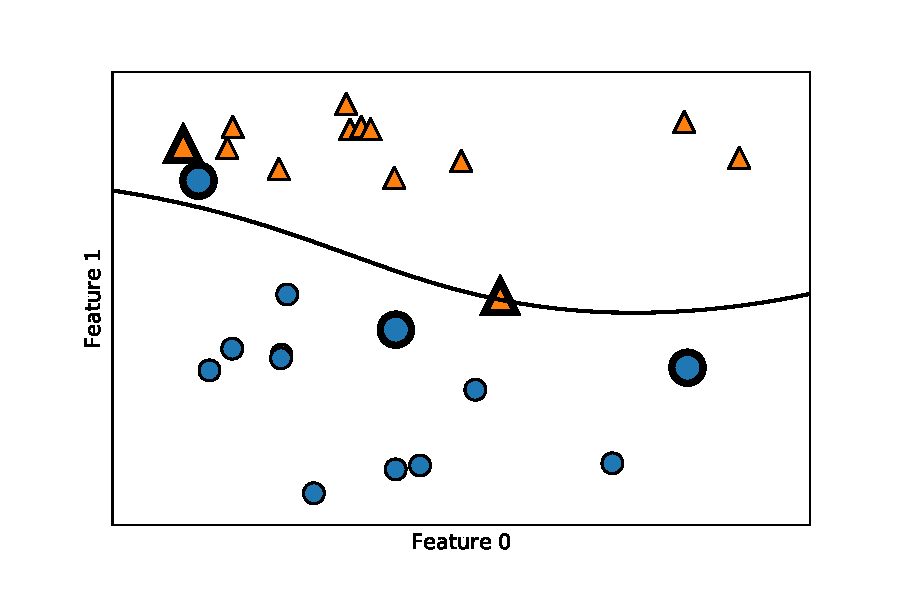
\includegraphics[width=\columnwidth]{images/Figure1.pdf}
  \caption{Decision Boundary and Support Vectors for Support Vector Machine 
  (SVM) with Nonlinear Kernel \cite{muller17}}
  \label{f:Figure1}
\end{figure}

%%%%%%%%%%%%%%%%%%%%%%%%%%%%%%%%%%%%%%%%%%%%%%%%%%%%%%%%%%%%%%%%%%%%%%%%%%%%%%%%

\emph{Support vector machines} (SVM) are an extension of SVC that use a 
kernel trick to reduce computational load. The radial basis function (RBF) 
kernel (i.e., Guassian kernel) is one of the most commonly used approaches. 
In training the model, only a subset of data points is used to construct the 
decision boundary, namely the support vectors that lie on the border that 
separates the two classes. In predicting classes for new observations, the 
algorithm calculates the distance to each of the support vectors measured 
by the Guassian kernel \cite{muller17}. Figure 1 shows an example of the 
non-linear decision boundary obtained with SVM using the RBF kernel; the 
decision boundary is a smooth curve and the support vectors are the large 
points in bold outline. Even with the default settings, the RBF kernel 
provides a decision boundary that is decidedly non-linear. The parameters 
for SVM are `C', which regulates the importance of each data point, and 
`gamma' which controls the width of the Guassian kernel. A small value of 
C indicates a restricted model in which the influence of each data point is 
limited and the algorithm adjusts to the majority of data points. With larger 
values of C, more importance is given to each data point and the model tries 
to correctly classify as many training observations as possible, which results 
in more curvature in the decision boundary. Large values of gamma mean that 
only close values are relevant for classification, resulting in a smooth 
decision boundary. Small values of gamma mean that far points are similar. 
If the values of both C and gamma are large, each point can have an large 
influence in a small region, which produces a choppy decision boundary. 
If the values of C and gamma are both small, the decision boundary becomes 
close to linear.

%%%%%%%%%%%%%%%%%%%%%%%%%%%%%%%%%%%%%%%%%%%%%%%%%%%%%%%%%%%%%%%%%%%%%%%%%%%%%%%%

The Bayes' rule was mentioned above in relation to LDA; in this section, the 
\emph{naive Bayes classifier} is considered as a non-linear model.
The Bayes theorem (equation 1) is represented by a set of probabilities to 
represent the following question: ``Based on a given set of predictors, what
is the probability than an outcome belongs to a particular class?''

\begin{equation}
  \ P(Y=cl|X) = \frac{P(Y)*P(X|Y=cl)}{P(X)}\
\end{equation}

The prior probability, P(Y), is the expected probability of a given class 
based on what is known (e.g., rate of disease in the population). P(X) 
is the probability of the predictor variables. The conditional probability,
$P(X=cl|Y)$, is the probability of observing the predictor variables for data 
associated with a given class. The naive Bayes model assumes that all of the 
predictor variables are independent, although this assumption is not always 
realistic. The conditional probabilities are calculated based on the 
probability densities for each individual predictor \cite{kuhn13}. For 
categorical predictors, the observed frequencies in the training set data 
can be used to determine the probability distributions. The prior probability 
allows us to tilt the final probability toward a particular class. Class 
probabilities are created and the predicted class is one associated with the 
largest class probability. Despite the somewhat unrealistic assumption of 
independence among predictors, the naive Bayes model is computationally quick, 
even with large training sets, and performs competitively compared to other 
models. The naive Bayes model encounters issues when dealing with frequencies 
or probabilities equal to zero, especially for small sample sizes. In addition, 
as the number of predictors increases relative to sample size, the posterior 
probabilities will become more extreme.

%%%%%%%%%%%%%%%%%%%%%%%%%%%%%%%%%%%%%%%%%%%%%%%%%%%%%%%%%%%%%%%%%%%%%%%%%%%%%%%%

\emph{Neural Networks} are powerful models for classification and 
regression based on theories of connectivity in the brain \cite{kuhn13}. 
The present study considers a simple method called multilayer perceptrons 
(MLP) as a feed-forward neural network \cite{muller17, raschka17}. 
The outcome is modeled by an intermediary set of unobserved variables called 
hidden units, which are linear combinations of the original predictors. 
Each hidden unit is a combination of some or all of the predictors which 
are then transformed by a nonlinear function (e.g., \emph{sigmoidal}). A 
neural network usually has multiple hidden units used to model the outcome. 
The MLP classifier computes weights between the inputs and the hidden layers, 
and weights between the hidden layers and the output. After computing each 
hidden unit, the output is modeled by a nonlinear combination of the hidden 
units. The nonlinear function allows the neural network to fit more 
complicated functions than a linear model. Neural networks are sensitive to 
the scaling of the features and can require extensive data preprocessing. 
There are several ways to modify the complexity of a neural network: by 
selecting the number of hidden layers, the number of units within each 
layer, and the regularization parameter (L2) which shrinks the weights 
towards zero. The feature weights provide an estimate of feature importance.
Although neural networks can capture information in large amounts of data 
with very complex models, they tend to overfit data used to train the model, 
and can be difficult to interpret. Neural networks may work best with 
homogenous datasets where the predictor variables all have similar meanings 
\cite{muhuri13}. For datasets with many different kinds of features, 
tree-based methods offer a better approach.

%%%%%%%%%%%%%%%%%%%%%%%%%%%%%%%%%%%%%%%%%%%%%%%%%%%%%%%%%%%%%%%%%%%%%%%%%%%%%%%%

\subsubsection{Tree-based Models} Decision trees are based on a hierarchy of 
\emph{`if-else'} questions starting from a root node and proceeding through a 
series of binary decisions or choices. Each node in the tree represents either 
a question or a terminal node (i.e., leaf) that contains the outcome. Applied to 
a binary classification task, the decision tree algorithm learns the sequence
of if-else questions that arrives at the outcome most quickly. For continuous 
features, questions are expressed in the form: ``Is feature x larger than 
value y?'' In constructing the tree, the algorithm searches through all 
possible tests and finds a solution that is most informative about the target 
outcome \cite{muller17}. The recursive branching process yields a binary tree 
of decisions, with each node representing a test for a single feature. This 
process of partitioning is repeated until each leaf in the decision tree 
contains only a single target. Prediction for a new data point proceeds by 
checking which region of the partition the point falls in, and predicting the 
majority in that feature space. The main advantage of tree models is that they 
require little adjustment and are easy to interpret. A drawback is that they 
can lead to complex models which are highly overfit to the training data. 
Prepruning`can help reduce overfitting by limiting the maximum depth of the 
tree, or the maximum number of leaves. Another approach is to set the minimum 
number of points in a node required for splitting. Decision trees work well 
with features measured on different scales, or with data that has a mix of 
binary and continuous features. 

%%%%%%%%%%%%%%%%%%%%%%%%%%%%%%%%%%%%%%%%%%%%%%%%%%%%%%%%%%%%%%%%%%%%%%%%%%%%%%%%

\emph{Random Forests} is an ensemble approach that combines many simple trees 
that each overfit the data in different ways. By building many trees and 
averaging their results, random forests helps to reduce overfitting. In 
constructing the forests, the user selects the number of trees to build 
(e.g., 1000). Randomness is introduced using a bootstrapping method that 
repeatedly draws random samples of size n from the data set (with replacement).  
The decision trees are build on these random samples of the same size, with 
some points missing and some data points repeated \cite{muller17,raschka17}.
The algorithm makes a random selection of p- features, and uses a different 
set of features at each node branch. These processes ensure that all of the 
decision trees in the random forest are different. Random forests is one of 
the most widely used supervised learning algorithms that works well without 
very much parameter tuning or scaling of data. A limitation is that Random 
forests do not perform well with high-dimensional data, or data that is 
sparse (e.g., text).

%%%%%%%%%%%%%%%%%%%%%%%%%%%%%%%%%%%%%%%%%%%%%%%%%%%%%%%%%%%%%%%%%%%%%%%%%%%%%%%%

\emph{Gradient Boosted trees} is another ensemble method that combines 
multiple decision trees in a serial fashion, where each tree tries to correct 
for mistakes of the previous one \cite{muller17}. Gradient boosted regression 
trees use strong pre-pruning, with shallow trees of a depth of one to five. 
Each tree only provides a good estimate of part of the data; combining many 
shallow trees (i.e., ``weak learners'') iteratively improves performance. 
In addition to pre-pruning and the number of trees, an important parameter 
for gradient boosting is the \emph{learning rate} which determines how 
strongly each tree tries to correct for mistakes of previous trees. A high 
learning rate produces stronger corrections, allowing for more complex models. 
Adding more trees to the ensemble also increases model complexity. Gradient 
boosting and random forests perform well on similar tasks and data. A common 
approach is to first try random forests and then include gradient boosting 
to improve model accuracy. 

%%%%%%%%%%%%%%%%%%%%%%%%%%%%%%%%%%%%%%%%%%%%%%%%%%%%%%%%%%%%%%%%%%%%%%%%%%%%%%%%

\begin{table}
  \caption{Confusion Matrix for Binary Classification.}
  \label{tab:freq}
  \begin{tabular}{llll}
    \toprule
     & &  Actual Outcome & \\
    \midrule
    Predicted & Outcome & No Misuse & PRL Misuse \\
    \midrule
    & No Misuse & \textbf{True Negative} & False Positive \\
    & & \textbf{(TN)} & (FP) \\
    \midrule
    & PRL Misuse & False Negative & \textbf{True Positive} \\
    & & (FN) & \textbf{(TP)}  \\
    \bottomrule
  \end{tabular}
\end{table}

%%%%%%%%%%%%%%%%%%%%%%%%%%%%%%%%%%%%%%%%%%%%%%%%%%%%%%%%%%%%%%%%%%%%%%%%%%%%%%%%

\subsection{Evaluating Model Performance}

It is necessary to evaluate the performance of different learning algorithms
in order to identify which model is best for a given problem with the data 
that is available. No model can make perfect predictions as there are always 
mistakes to be found. Binary classification is assessed in terms of the 
successful assignment of observations to one of two classes: positive or 
negative. Medical testing provides a useful example to illustrate 
classification decisions and errors: A patient can actually have an illness 
or not and the person is either diagnosed as having the illness or not. In 
the present case, the positive class represents self-reported pain reliever 
misuse and abuse (PRLMISAB), and predictions based on the classifier models 
will be either correct or incorrect in relation to the observed outcomes. 
For example, a person who has never misused or abused pain relievers may be 
misclassified as having done so (i.e., 'false positive'), or conversely, a 
a person who actually has misused and abused pain relievers may be labeled 
as never having done so (i.e., 'false negative').

%%%%%%%%%%%%%%%%%%%%%%%%%%%%%%%%%%%%%%%%%%%%%%%%%%%%%%%%%%%%%%%%%%%%%%%%%%%%%%%%

Correct decisions and classification errors are represented in a 
\emph{confusion matrix} (Table 1) that indicates the correspondence between 
predicted and actual outcomes. The confusion matrix is a two-by-two array in 
which the columns correspond to the actual observed classes and the rows 
correspond to the predicted classes. The main diagonal indicate the number of 
correctly classified samples (\emph{true positive, true negative}), while the 
other entries represent the number of samples in one class that were mistakenly 
classified as another class. Several measures of preformance can be obtained
from the confusion matrix, including accuracy, sensitivity (i.e., recall), 
specificity, precision, and the $f_1$-score (Table 2) \cite{kuhn13, wiki18}. 
Model performance is most commonly evaluated using \emph{Accuracy} which is 
assessed by the number of correct predictions divided by the total number 
of observations. Sensitivity or \emph{Recall} provides the ``True Positive 
Rate'' (TPR), measured as the number of positive samples that are correctly 
identified by the prediction (number of sick patients correctly diagnosed). 
Recall is used when the goal is to avoid false negatives. The True Negative 
Rate (TNR) is described as Specificity, which indicates the proportion of 
negative cases correctly identified (healthy people not misdiagnosed). 
\emph{Precision} provides the ``Positive Predictive Value'' (PPV), which 
measures how many of the samples predicted as positive are actually positive. 
Precision is used as a metric when the goal is to limit the number of false 
positives. The \emph{$f_1$-score} or `f-measure' represents a harmonic mean 
between recall and precision (\(\frac{2}{ \frac{1}{R} + \frac{1}{P} }\) ).
The $f_1$-score can be a better performance metric than accuracy 
in datasets with imbalanced classes, where one class is much more frequent 
than the other class, as it takes into account both recall and precision 
\cite{muller17, yun09}.

%%%%%%%%%%%%%%%%%%%%%%%%%%%%%%%%%%%%%%%%%%%%%%%%%%%%%%%%%%%%%%%%%%%%%%%%%%%%%%%%

\begin{table}
  \caption{Performance Metrics for Classifier Models.}
  \label{tab:freq}
  \begin{tabular}{lc}
    \toprule
    Accuracy & \(\frac{TP+TN}{TP+FP+TN+FN}\) \\
    & \\
    Sensitivity, Recall (TPR) &  \(\frac{TP}{TP+FN}\) \\
    & \\
    Specificity (TNR) &  \(\frac{TN}{TN+FP}\) \\
    & \\
    Precision (PPV) & \(\frac{TP}{TP+FP}\)  \\
    & \\
    f_1 score & 2*\(\frac{Precision*Recall}{Precision+Recall}\) 
    & \\
    \bottomrule
  \end{tabular}
\end{table}

%%%%%%%%%%%%%%%%%%%%%%%%%%%%%%%%%%%%%%%%%%%%%%%%%%%%%%%%%%%%%%%%%%%%%%%%%%%%%%%%

\begin{figure}[!ht]
  \centering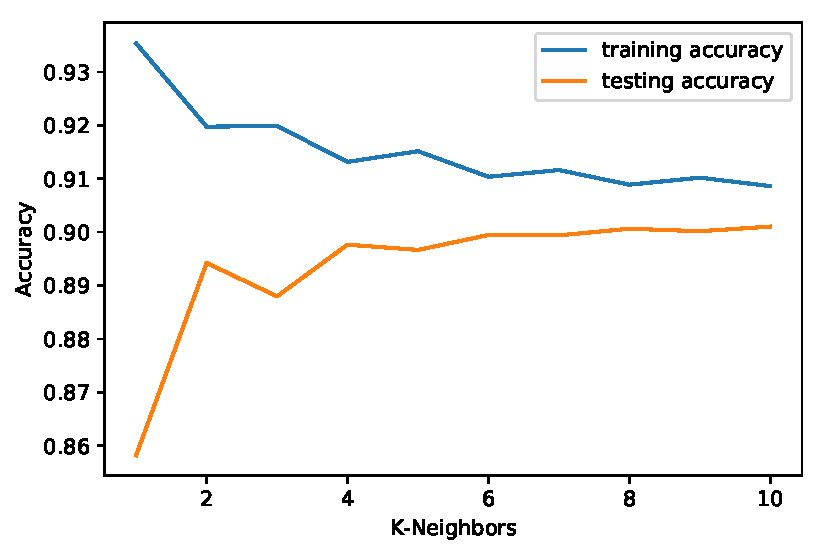
\includegraphics[width=\columnwidth]{images/Figure2.pdf}
  \caption{K-Nearest Neighbors Classifier Accuracy for Training Set and 
  Testing Set as a function of Number of Neighbors.}
  \label{f:Figure2}
\end{figure}

%%%%%%%%%%%%%%%%%%%%%%%%%%%%%%%%%%%%%%%%%%%%%%%%%%%%%%%%%%%%%%%%%%%%%%%%%%%%%%%%

\begin{table*}[ht]
  \caption{Variables Included in the Sample Data for Model Construction.}
  \label{tab:freq}
  \begin{tabular}{ll}
    \toprule
    \textit{Target Outcome} & Label \\
    \midrule
    Prescription Opioid Pain Reliever Misuse and Abuse 
    (Likert scale: 0-12)& PRLMISAB  \\
    \midrule
    \textit{Predictor Variables}&   \\
    \midrule
    Year of NSDUH Survey (15=2015, 16=2016, 17=2017) & YEAR  \\
    Age Category (1=12-17 years, 2=18-25, 3=26-35, 4=36-49, 5=50 and older)& AGECAT \\
    Biological Sex (0=Male, 1=Female)& SEX  \\
    Marital Status (0=Unmarried, 1=Divorced, 2=Widowed, 3=Married)& MARRIED  \\
    Education (1=H.S. or Less, 2=H.S. Grad., 3=Some College,  4=College Grad.)& EDUCAT  \\
    Employment Status (Over 18: 1=Not Employed, 2=Part-time, 3=Full-time) & EMPLOY18  \\
    Size of City/Metropolitan Region (1=Rural, 2=Small, 3=Large)& CTYMETRO  \\
    Health Problems Aggregated  (Likert scale: 0-10)& HEALTH  \\
    Mental Health, Aggregated: adult depression, emotional distress 
    (Likert scale: 0-10)& MENTHLTH  \\
    Treatment for Drugs and Alcohol in past year, Aggregated 
    (Likert scale: 0-5)& TRTMENT  \\
    Mental Health Treatment, Aggregated (Likert scale: 1-10)& MHTRTMT  \\
    Tranquilizer use, past year, Aggregated (Likert scale: 0-5)& TRQLZRS \\
    Sedative use, past year, Aggregated (Likert scale: 0-5)& SEDATVS  \\
    Heroin use, past year, Aggregated (Likert scale: 0-5)& HEROINUSE  \\
    Cocaine and Crack Cocaine Use in past year, Aggregated  
    (Likert scale: 0-5)& COCAINE  \\
    Amphetamine and Methamphetamine Use in past year, Aggregated 
    (Likert scale: 0-5)& AMPHETMN  \\
    \bottomrule
  \end{tabular}
\end{table*}

%%%%%%%%%%%%%%%%%%%%%%%%%%%%%%%%%%%%%%%%%%%%%%%%%%%%%%%%%%%%%%%%%%%%%%%%%%%%%%%%

\subsubsection{Training and Test Set Accuracy}

In constructing and evaluating predictive models it is important to select 
a model that performs well not only with the data used to train the model, 
but also with new observations. A standard practice is to divide the sample 
data into a \emph{training set} and a \emph{testing set} of observations that 
is set aside and used to evaluate model performance. By convention, approximately 
70 to 80 percent of observations are used in the training set and the remaining 
portion is held in the testing set. Two main problems can occur in evaluating 
model performance: overfitting and underfitting. In the case of 
\emph{overfitting}, A model can have high accuracy on the training set 
but perform poorly with new data in the test set because the model is 
`over-fit' to the training data. By contrast, a model can attain high 
accuracy with the test set, while performing poorly with the training data 
because of \emph{underfitting}. One of the simplest classification models, 
K-Nearest neighbors provides an illustrative example. KNN classifies 
observations by assigning the label that is most frequent among the `k' 
number of nearest training samples (k is a parameter selected by the user). 
The accuracy of the KNN classifier for the training set and testing set is 
plotted as a function of the parameter k-neighbors in Figure 2. The plot 
shows that increased accuracy on the testing set is associated with 
decreased training set accuracy, and conversely, increase accuracy on 
the training set is related to decreased test set accuracy. The best model 
optimizes test set accuracy while strikes a balance between the problems of 
overfitting and underfitting. In the case of KNN, performance on the test set 
increased only slightly between 2 and 4 neighbors, but did not improve much 
beyond 5 neighbors. Therefore, a model with k=4 neighbors provides a 
reasonable solution for the data. 

\subsubsection{Imbalanced Classes}

Previous studies have analyzed the misuse and abuse of prescription opioids
(MUPO) using logistic regression and identified factors that influence MUPO 
such as gender and mental illness \cite{rice12, unick13, jones15, mccabe12}. 
The present study extends previous work by comparing the performance of ten 
classifier models of pain reliever misuse and abuse and evaluating each model 
using four performance metrics (accuracy, sensitivity, precision, $f_1$-score). 
The sample data set has imbalanced classes in the target variable as instances 
of one class (negative) greatly outnumber instances of the other class. 
A difficulty of using traditional classification algorithms with imbalanced 
data is that they tend to classify observations as belonging to the majority 
class when the class of interest (positive) is represented by the minority of 
observations \cite{brown12, yun09}. This can produce a result which 
underestimates the occurence of positive cases which are misclassified as 
false negatives. Efforts to address the issue of imbalanced data have included 
sampling methods such as `boosting'. As described above, the $f_1$-score is 
a better measure of performance than accuracy with data that have imbalanced 
classes as it takes into account both sensitivity (i.e., recall) and precision. 
The study also identifies features important for predicting MUPO. The tradeoffs 
between model performance and model interpretability is discussed. 

%%%%%%%%%%%%%%%%%%%%%%%%%%%%%%%%%%%%%%%%%%%%%%%%%%%%%%%%%%%%%%%%%%%%%%%%%%%%%%%%

\section{Method}

\subsection{The Data}

The NSDUH public data files for 2015, 2016, and 2017 were downloaded from 
the Substance Abuse and Mental Health Data Archive (SAMHDA) \cite{samhsa18}. 
The data sets were extracted and saved as data frame objects in a python 
interactive notebook \cite{mckinney17, vanderplas17}. Data from the three
years ($n_1$=57146, $n_2$=57897, $n_3$=56276) were combined to create a 
total sample consisted of N=170317 observations (80913 male, 89404 female). 
According to the NSHUD codebook, the sampling design is weighted across 
states by population size, drawing more heavily from eight states with 
the largest populations (e.g., CA, FL, IL, MI, NY, OH, PA, TX), for a 
representative distribution that accounts for approximately 48 percent 
of the U.S. population. For 2015, the weighted survey screening response 
rate was 81.94\% and the weighted interview response rate was 71.2\% 
\cite{samhsa18}. Identifying information in the public use files is 
collapsed (e.g., age categories); variables related to ethnicity, immigration 
status, and state identifiers are removed to ensure confidentiality. The data 
frames were subset by column to select approximately 90 variables that 
included common demographic characteristics, physical health, mental health, 
medication usage, and illicit drug use. Inconsistencies in the data were 
detected and removed by the following steps: (a) Remove missing values 
(i.e., NaN); (b) Recode blanks, non-responses, or legitimate skips 
(e.g., 99, 991, 993) to zero; (c) Recode dichotomous responses (e.g., No=0, 
Yes=1); (d) Recode categorical variables to be consistent with amount or 
degree  (e.g., 1=`Low', 2=`Med', 3=`High'). (e) Identify and remove 
outliers (n=2).

%%%%%%%%%%%%%%%%%%%%%%%%%%%%%%%%%%%%%%%%%%%%%%%%%%%%%%%%%%%%%%%%%%%%%%%%%%%%%%%%

\begin{table}
  \caption{Frequency of Pain Reliever Misuse and Abuse
  by Demographics Features for NSDUH 2015-2017 Sample.}
  \label{tab:freq}
  \begin{tabular}{llllll}
    \toprule
              & PRL Misuse & & & No Misuse & \\
              & N & \% &  & N & \% \\
    \midrule
    \textbf{Total}     & 18237 & 10.7\% & & 152080 & 89.3\% \\
    Male      & 9279 & 50.9\% & & 71634 & 47.1\%  \\
    Female    & 8958 & 49.1\% & & 80446 & 52.9\%  \\
    \midrule
    \textbf{Age Group} &  &  &  &  & \\
    12-17     & 2262 & 12.4\% & & 39315 & 25.9\% \\
    18-25     & 5577 & 30.6\% & & 36476 & 24.0\% \\
    26-35     & 4370 & 24.0\% & & 22251 & 14.6\% \\
    36-49     & 4173 & 22.0\% & & 29571 & 19.4\% \\
    50+       & 1855 & 10.2\% & & 24467 & 16.1\% \\
    \midrule
    \textbf{Education} Level &  &  &  &  & \\
    School Age & 2262 & 12.4\% & & 39315 & 25.9\% \\
    Some H.S.  & 1849 & 10.1\% & & 10507 & 10.1\% \\
    H.S. Grad  & 4134 & 22.7\% & & 20290 & 19.9\% \\
    Some Coll. & 5997 & 32.9\% & & 24922 & 24.5\% \\
    Coll. Grad & 3995 & 21.9\% & & 19726 & 19.7\% \\
    \midrule
    \textbf{Marital Status} &  &  &  &  & \\
    Single    & 6777 & 37.2\% & & 64022 & 42.1\% \\
    Divorced  & 6497 & 35.6\% & & 46183 & 30.4\% \\
    Widowed   & 1225 &  6.7\% & &  7995 &  5.3\% \\
    Married   & 3738 & 20.5\% & & 33880 & 22.3\% \\
    
    \bottomrule
  \end{tabular}
\end{table}

%%%%%%%%%%%%%%%%%%%%%%%%%%%%%%%%%%%%%%%%%%%%%%%%%%%%%%%%%%%%%%%%%%%%%%%%%%%%%%%%

\subsubsection{Aggregated Variables}

Related features were combined to created aggregated variables. For example, 
a single variable indicating overall history of health problems (`HEALTH`) 
was created by combining responses for overall health (reverse scored), any
previous diagnosis of STDs, hepatitis, HIV, cancer, and any hospitalization. 
A mental health variable (`MENTHLTH') aggregated responses for adult depression, 
emotional distress, suicidal thoughts or plans. Binary responses for ten of 
the most commonly used prescription pain medications (e.g., Hydrocodone, 
Oxycodone, Tramadol, Morphine, Fentanyl, Oxymorphone, Demerol, Hydromorphone) 
were aggregated into a variable for any prescription opioid pain reliever use 
(ANYPRLUSE) in the past year. The majority of questions related to substance 
use had dichotomous responses that were summed to create single measures for: 
Tranquilizers, Sedatives, Heroin, Cocaine, and Amphetamines. Because 
hallucinogens varied greatly in type and potency (e.g., marijuana, psilocybin, 
MDMA, LSD), they were not included in the analysis. Variables for drug 
treatment and mental health treatment combined responses for any inpatient 
care, outpatient care, treatment at a clinic, emergency room visits, or 
hospital stays. The target variable was any prescription opioid pain reliever 
misuse or abuse (PRLMISEVR). The subset data frame consisted of 19 features 
and 170317 observations was exported to CSV file. Four variables were highly 
correlated with other variables and excluded from the analysis (PRLANY, PRLMISAB, 
HEROINUSE, HEROINFQY). Table 2 shows the list of predictor variables used for 
constructing the classification models. 

%%%%%%%%%%%%%%%%%%%%%%%%%%%%%%%%%%%%%%%%%%%%%%%%%%%%%%%%%%%%%%%%%%%%%%%%%%%%%%%%

\subsubsection{Model Construction and Evaluation}

The dataset was divided using a 75 to 25 percent split to create the training 
set ($n_1$=127738) and testing set ($n_2$=42579). The same general procedure 
was used for constructing and evaluating each classification model: (i) The 
model was fit to the training set; (ii) New values were predicted on the 
holdout scores in the testing set; and (iii) Model performance on the test 
set was evaluated in a confusion matrix. The performance metrics of accuracy, 
sensitivity or recall, precision, and $f_1-score$ were obtained or derived 
from the confusion matrix. The logistic regression classifier, LDA, QDA, 
decision trees classifier, random forests classifier, gradient boosted trees 
were constructed using the caret package. The KNN classifier, support 
vector classifier (SVC), naive Bayes classifier, and neural network 
(multilayer perceptron) were built using scikit-learn. 

%%%%%%%%%%%%%%%%%%%%%%%%%%%%%%%%%%%%%%%%%%%%%%%%%%%%%%%%%%%%%%%%%%%%%%%%%%%%%%%%

\begin{figure}[!ht]
  \centering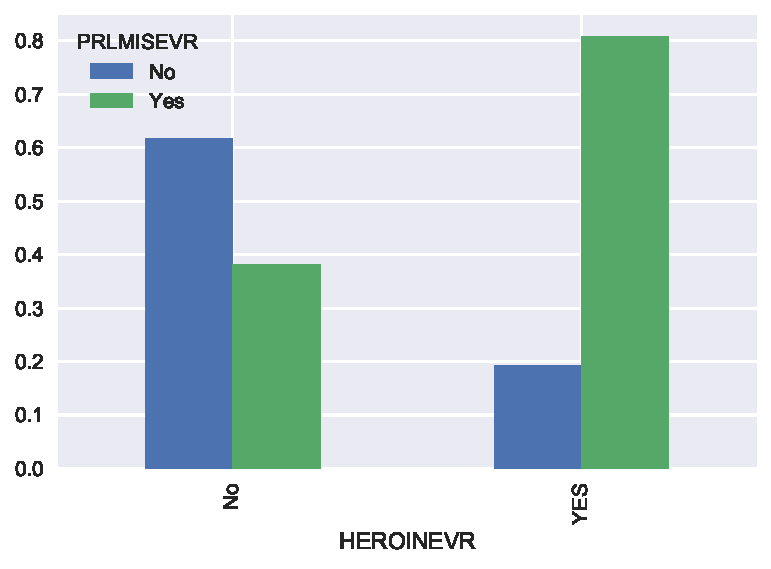
\includegraphics[width=\columnwidth]{images/Figure3.pdf}
  \caption{Proportion of Pain Reliever Misuse and Abuse
  as a function of Heroin Use.}
  \label{f:Figure3}
\end{figure}

%%%%%%%%%%%%%%%%%%%%%%%%%%%%%%%%%%%%%%%%%%%%%%%%%%%%%%%%%%%%%%%%%%%%%%%%%%%%%%%%

\section{Results}

\subsection{Exploratory Data Analysis}

Twenty-six percent of the total sample (n=44596) reported taking any pain 
relievers in the past year (19558 males, 25038 females). 
Table 4 provides the frequency and percent of respondents who reported 
pain reliever misuse and abuse by demographic characteristics. 
Approximately 11\% of the sample had misused or abused prescription pain 
relievers at some point; this same rate of pain reliever misuse and abuse 
was found in both the training set and test sets. Although a larger
number of females reported using any prescription opioid pain relievers in 
the past year than males, more males reported misusing or abusing opioid 
pain relievers. Pain reliever misuse was most frequent among individuals who 
described themselves as single, divorced, or with some college education. 
The proportion of pain reliever misuse and abuse was highest among 
individuals between 18 to 25 years of age and decreased among older age 
groups. Two percent of respondents (n=3433) disclosed ever using heroin 
(2019 males; 1414 females). As shown in Figure 3, among respondents who 
reported using pain relievers in the past year, the rate of misuse and abuse 
of pain relievers was twice as large for individuals who reported using 
heroin than those who had not used heroin, which is consistent with 
past findings that indicate a connection between MUPO and heroin use 
\cite{muhuri13, unick13}.
 
%%%%%%%%%%%%%%%%%%%%%%%%%%%%%%%%%%%%%%%%%%%%%%%%%%%%%%%%%%%%%%%%%%%%%%%%%%%%%%%%
 
\subsection{Classifier Model Performance}

Performance of the classification models was evaluated in the confusion 
matrices reported in Table 6, which includes the metrics of accuracy, 
sensitivity (recall), precision, and $f_1$-score. The model accuracy 
scores ranged form 86.1\% to 90.6\%. Because of unbalanced classes in 
the sample data | the proportion of respondents who had never misused or 
abused pain relievers (89\%) was much greater than the proportion who had | 
the $f_1$-score was used as the preferred metric of performance rather 
than accuracy as it takes into account both recall and precision. The 
$f_1$-scores ranged form 0.88\% to 0.946\%. Although the neural networks 
(MLP) model and support vector classifier (SLC) had the highest accuracy 
(90.6\% and 90.4\%, respectively), they both had very low $f_1$-scores 
compared to other models (0.88). In terms of the $f_1$-score, logistic 
regression, decision trees, and random forests performed better than 
other classifiers and were tied for the highest score (0.946). The 
random forests model identified more true positives than a single decision 
tree and had fewer misclassification errors than the logistic regression 
model. The main parameter settings for the classification models are 
presented in Table 7.
 
%%%%%%%%%%%%%%%%%%%%%%%%%%%%%%%%%%%%%%%%%%%%%%%%%%%%%%%%%%%%%%%%%%%%%%%%%%%%%%%%

\begin{table}
  \caption{Parameter Estimates for Logistic Regression Model and Log-odds 
  Ratios for Pain Reliever Misuse and Abuse (Training Set).}
  \label{tab:freq}
  \begin{tabular}{lllll}
    \toprule
    Predictor&  Estimate& Std. Err.& Z-Value & Odds Ratio \\    
    \midrule
    (Intercept)   & -1.901 &  0.307 &  -6.19 *** &   \\
    Cocaine       &  0.672 &  0.015 &  44.43 *** & 1.96  \\
    Amphetamines  &  0.592 &  0.017 &  35.55 *** & 1.81  \\
    Tranquilizers &  0.393 &  0.011 &  34.57 *** & 1.48  \\
    Mental Health &  0.133 &  0.005 &  26.96 *** & 1.14  \\
    Heroin use    &  0.750 &  0.041 &  18.25 *** & 2.12  \\
    Age Category  & -0.185 &  0.011 & -17.28 *** & 1.20  \\
    Employment    &  0.191 &  0.013 &  14.60 *** & 1.21  \\
    Treatment     &  0.203 &  0.015 &  13.57 *** & 1.23  \\
    Sedatives     &  0.264 &  0.024 &  10.98 *** & 1.30  \\
    Education     &  0.105 &  0.010 &  10.12 *** & 1.11  \\
    Health        &  0.093 &  0.010 &   9.15 *** & 1.10  \\
    Sex           & -0.153 &  0.021 &  -7.28 *** & 1.17  \\
    Married       &  0.052 &  0.010 &   5.42 *** & 1.05  \\
    Year          & -0.071 &  0.020 &  -3.58 *** & 1.07  \\
    City/Metro    & -0.040 &  0.013 &  -3.08 **  & 1.04  \\
    MH Treatment  & -0.001 &  0.014 &  -0.07     & 1.00  \\
    \bottomrule 
    Note: p-value& $<$ 0.001***  & $<$ 0.01** &  &   
  \end{tabular}
\end{table}


%%%%%%%%%%%%%%%%%%%%%%%%%%%%%%%%%%%%%%%%%%%%%%%%%%%%%%%%%%%%%%%%%%%%%%%%%%%%%%%%
 
\begin{table*}[ht]
  \caption{Confusion Matrices and Performance Metrics for Predictive Models of 
  Pain Reliever Misuse and Abuse}
  \label{tab:freq}
  \begin{tabular}{llllllll}
    \toprule
    Model& & Confusion Matrix & & Accuracy & Sensitivity & Precision & F1-Score \\
    \midrule
    K-Nearest Neighbors & & No Misuse & PRL Misuse &  &  &  & \\
     & No Misuse & 37595 & 426 & 89.8\% & 0.900 & 0.870 & 87\% \\
     & PRL Misuse & 3909 & 650 &  &  &  & \\
    \midrule
    Logistic Regression & & No Misuse & PRL Misuse &  &  &  & \\
     & No Misuse & 37618 & 3478 & 90.7\% & 0.987 & 0.915 & 95\% \\
     & PRL Misuse &  495 &  988 &  &  &  & \\
    \midrule
    Linear Discriminant Analysis (LDA) & & No Misuse & PRL Misuse &  &  &  & \\
     & No Misuse & 37063 & 3073 & 90.3\% & 0.973 & 0.923 & 94.7\% \\
     & PRL Misuse & 1050 & 1393 &  &  &  & \\
    \midrule
    Quadratic Discriminant Analysis (QDA) & & No Misuse & PRL Misuse &  &  &  & \\
     & No Misuse & 34786 & 2426 & 86.5\% & 0.913 & 0.935 & 92.4\% \\
     & PRL Misuse & 3327 & 2040 &  &  &  & \\
    \midrule
    Support Vector Classifier (SVM) & & No Misuse & PRL Misuse &  &  &  & \\
     & No Misuse & 37681 & 340 & 90.3\% & 0.900 & 0.890 & 88\% \\
     & PRL Misuse & 3787 & 772 &  &  &  & \\
    \midrule
    Naive Bayes & & No Misuse & PRL Misuse &  &  &  & \\
     & No Misuse & 38110 & 4431 & 89.6\% & 0.999 & 0.896 & 94.5\% \\
     & PRL Misuse & 3 & 35 &  &  &  & \\
    \midrule
    Neural Network (MLP) & & No Misuse & PRL Misuse &  &  &  & \\
     & No Misuse & 37563 & 458 & 90.1\% & 0.90 & 0.88 & 88\% \\
     & PRL Misuse & 3682 & 877 &  &  &  & \\
    \midrule
    Decision Trees & & No Misuse & PRL Misuse &  &  &  & \\
     & No Misuse & 376552 & 3597 & 90.5\% & 0.988 & 0.913 & 94.9\% \\
     & PRL Misuse &   458 &  869 &  &  &  & \\
    \midrule
    Random Forests & & No Misuse & PRL Misuse &  &  &  & \\
     & No Misuse & 25026 & 2298 & 90.1\% & 0.987 & 0.909 & 95\% \\
     & PRL Misuse & 320 & 665 &  &  &  & \\
    \midrule
    Gradient Boosted Trees & & No Misuse & PRL Misuse &  &  &  & \\
     & No Misuse & 37956 &  65 & 89.8\% & 0.90 & 0.89 & 89.5\% \\
     & PRL Misuse & 4261 & 298 &  &  &  & \\
    \bottomrule
  \end{tabular}
\end{table*}

%%%%%%%%%%%%%%%%%%%%%%%%%%%%%%%%%%%%%%%%%%%%%%%%%%%%%%%%%%%%%%%%%%%%%%%%%%%%%%%%
 
\begin{table}
  \caption{Main Parameters for Non-linear Classification Models of 
  Pain Reliever Misuse and Abuse}
  \label{tab:freq}
  \begin{tabular}{ll}
    \toprule
    Model & Main Parameter \\
    \midrule
    K-Nearest Neighbors & Number of Neighbors = 4 \\
    Naive Bayes & Cost, \textit{C} = 0.01 \\
    Neural Network & Hidden Layers = 1 \\
    Decision Trees & Maximum Depth = 4 \\ 
    Random Forests & Number of Trees = 1000 \\
    Boosted Trees & Learning Rate = 0.01 \\ 
    \bottomrule
  \end{tabular}
\end{table}

%%%%%%%%%%%%%%%%%%%%%%%%%%%%%%%%%%%%%%%%%%%%%%%%%%%%%%%%%%%%%%%%%%%%%%%%%%%%%%%%

\subsubsection{Logistic Regression}

The parameter estimates and odds ratios for the logistic regression model are 
presented in Table 5, sorted by z-score. The ceofficient estimates for all of 
the features were statistically significant ($p<.001$), with the exception of 
mental health treatment. The coefficient estimates ($\beta_i$...$\beta_j$) 
are interpreted as the change in the log of the odds of the dependent variable 
(PRLMISAB) occurring given a one unit change in each independent variable
($X_i$...$X_j$), holding constant the effects of other independent variables. 
The parameters relate to the log of the odds ratio rather than to the dependent 
variable directly. The odds are calculated as the probability of the event 
occurring divided by the probability of the event not occurring 
( \(\frac{P}{P-1}\) ). The odds ratios are obtained by taking the antilog of 
the estimated coefficients, which are the exponentiated parameter estimates 
($e^x$). For an interval scaled independent variable, the odds ratio 
is interpreted as the multiplicative increase in the odds of the dependent 
variable event happening given a one unit change in the value of the 
independent variable, assuming the effects of all other independent variables 
are held constant. For a dichotomous (dummy) independent variable, e.g., sex, 
the multiplicative increase in the odds of the dependent variable event 
happening if the event represented by the independent variable occurs, holding 
constant the effects of all other independent variables. In general, if you 
take the antilog of the coefficient estimate, subtract 1 from it, and multiply 
the result by 100, you get the percent change in the odds for a unit increase 
in the independent variable  \cite{gujarati09}.  The odds ratio indicates the 
ratio of the positive event to negative event, but does not reveal the 
probability of the positive outcome.

%%%%%%%%%%%%%%%%%%%%%%%%%%%%%%%%%%%%%%%%%%%%%%%%%%%%%%%%%%%%%%%%%%%%%%%%%%%%%%%%

The odds ratios presented in Table 5 can be interpreted as the odds of a 
respondent misusing or abusing pain relievers increases by 1.99 times or 99\% 
for a one unit increase in cocaine use, holding the effects of all other 
independent variables constant. 

For a one unit increase in amphetamine use, 
the odds of pain reliever misuse and abuse (PRLMISAB) increases by 1.84 times
or 84\%, holding all other IVs constant. A one unit increase in tranquilizer 
use is associated with a 1.46 or 46\% increase in the odds of PRLMISAB, 
holding other IVs constant. For a unit increase in mental health issues, the
odds for PRLMISAB increased by 1.15 or 15\%. For a one unit increase in age 
category, the odds of PRLMISAB decreased by 1.24 times or 24\%, holding the 
effects of other IVs constant. For a one unit increase in heroin use, the odds 
of PRLMISAB increases by 2.22 times or 22\%, holding other IVs constant. A one 
unit increase in employment is associated with a 1.25 or 25\% increase in the 
odds of PRLMISAB, holding other IVs constant. For a unit increase in substance 
treatment, the odds for PRLMISAB increased by 1.22 or 22\%, holding other IVs 
constant. For a one unit increase in sedative use, the odds of PRLMISAB 
increases by 1.32 times or 32\%, holding all other IVs constant. For a one 
unit increase in health problems, the odds for PRLMISAB increased by 1.11 or
11\%, holding other IVs constant. For a one unit increase in education, the 
odds of PRLMISAB increased by 1.11 times or 11\%, holding other IVs constant. 
In terms of sex, the odds of misusing or abusing pain relievers for females 
decreases by 1.20 times compared to males, holding all other IVs constant. 
In other words, the odds of PRLMISAB for females was 20\% lower than for males. 
A unit increase in the size of a respondents city or metropolitan area 
resulted in a 1.07 or 7\% decrease in the odds of PRLMISAB, holding other 
IVs constant. For a unit increase in marital status, the odds for PRLMISAB 
increases by 1.05 or 5\%, holding other IVs constant. 
 
%%%%%%%%%%%%%%%%%%%%%%%%%%%%%%%%%%%%%%%%%%%%%%%%%%%%%%%%%%%%%%%%%%%%%%%%%%%%%%%%

\subsubsection{Decision Trees} 

The decision tree model was prepruned to a maximum depth of 4, which means 
the algorithm split on four consecutive features (see Figure 4). The  
algorithm selected cocaine as the root node which includes the 85528 
observations in the training set. With a classification tree, we predict 
that each observation will belong to the class of training observations in 
the region to which it belongs, and want to determine not only the class
prediction belonging to a terminal node region, but also the class 
proportions among the training observations in that region \cite{james13}. 
One way to interpret a decision tree is by following the number of samples 
represented at the split for each node. Another way to interpret the decision 
tree in Figure 4 is by the examining the proportion of observations of 
class A captured by that leaf over the entire number of observations captured 
by the leaf during model training. Starting from the root node the branch 
to the left represents 75562 observations with no or low cocaine use; 
of those, 0.07 or 7\% reported misusing or abusing opioid pain relievers. 
Following the right branch are 9966 observations positive for cocaine use, 
of which 0.39 or 39\% reported pain reliever misuse or abuse. In other words, 
the proportion of pain reliever misuse and abuse was more than five times as 
large for individuals who reported using cocaine than those who had not. 

\begin{figure}[!ht]
  \centering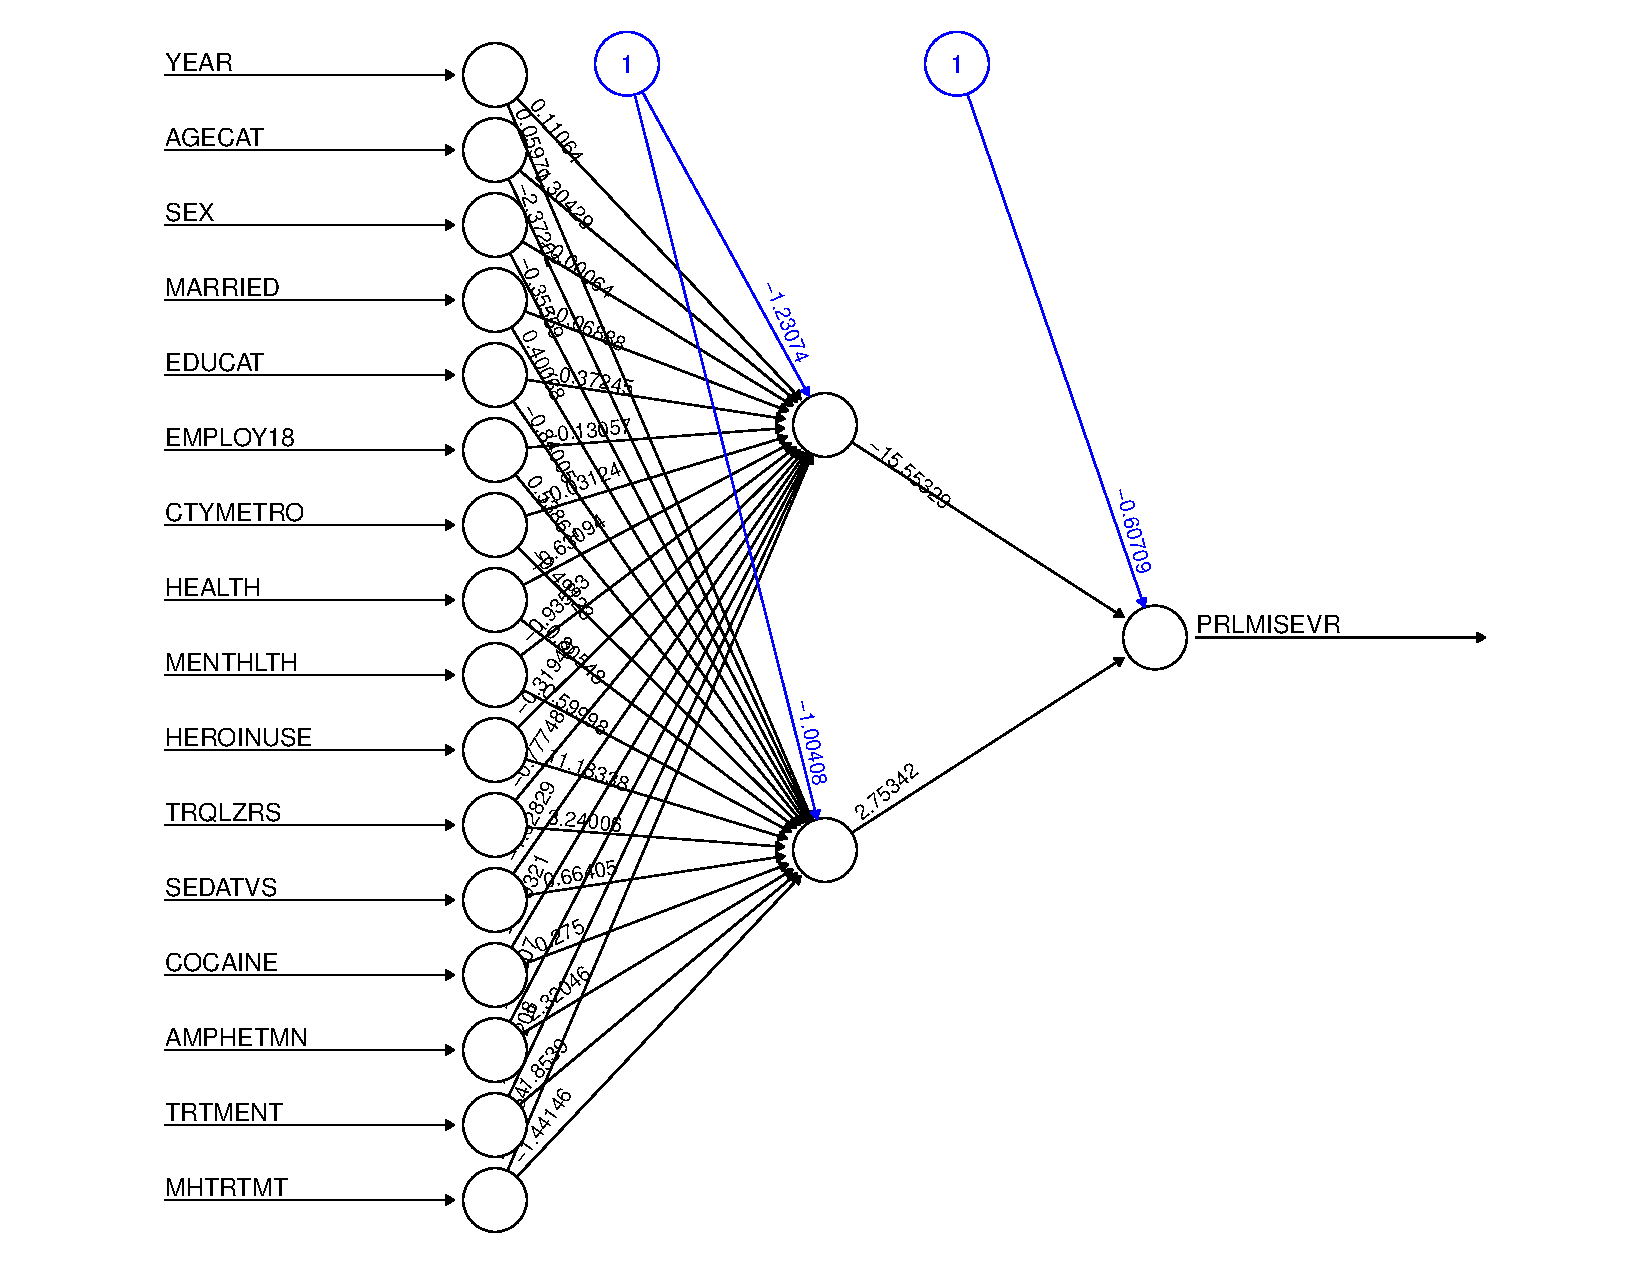
\includegraphics[width=\columnwidth]{images/Figure5.pdf}
  \caption{Decision Tree Model of Pain Reliever Misuse and Abuse
  fit to the Training Set}
  \label{f:Figure5}
\end{figure}

The second split was based on heroin use which included 9966 observation; 
to the left branch were 8562 respondents who had not used heroin, of which
0.34 or 34\% reported PRLMISAB. Following the right branch to the terminal 
node (i.e., `leaf') were 1404 individuals positive for heroin use, of which
0.70 or 70\% had misused or abuse pain relievers. Thus, the proportion of 
PRLMISAB was twice as large for respondents who had used heroin than those 
who had not (as seen in Figure 3). The third split in the decision tree was 
based on tranquilizers, which included 8562 observations. On the left branch 
were 6455 observation with no or low tranquilizer use; of these, the 
proportion of PRLMISAB was 0.28 or 28\%. To the branch on the right were 
2016 observations with higher tranquilizer use, of which 0.51 or 51\% 
reported PRLMISAB. Similar to what was observed in the case of heroin, the 
rate of pain reliever misuse and abuse for individuals with moderate to high
tranquilizer use was almost twice as large than for those with no to low
tranquilizer use. The fourth split was based on age category which included
2107 observations; the branch to the left represented 946 individuals age 
36 or older, of which 0.35 or 35\% reported PRLMISAB. The branch to the 
right represented 1162 individuals age 35 and younger, of whom 0.64 or 64\% 
reported PRLMISAB. The proportion of pain reliever misuse and abuse for
respondents 35 or younger was almost twice that as individuals older 
than 35 years of age. 

%%%%%%%%%%%%%%%%%%%%%%%%%%%%%%%%%%%%%%%%%%%%%%%%%%%%%%%%%%%%%%%%%%%%%%%%%%%%%%%%
\subsubsection{Feature Importance for Random Forests}

The random forest model was fit using 1000 trees, with all of the features 
considered at each node to determine the randomness of each tree. After a 
large number of trees is generated, each tree represents a vote for the
most popular class. Although random forests perform well with data that has
imbalanced classes, it can be difficult to interpret the result of the 
averaged trees. Feature importance is a model summary for random forests 
that rates how important each feature is for classification decisions made 
in the algorithm. The Gini index provides a measure of node purity which is 
used to evaluate the quality of a particular split; a small value indicates 
that a node predominantly contains observations from a single class. 
Feature importance was measured by the mean decrease in Gini coefficient 
(see Table 8), which indicates how each variable contributes to the 
homogeneity of the nodes and leaves in the resulting random forest. 
For classification trees, the splits are chosen so as to minimize entropy 
or Gini impurity in the resulting subsets. For random forests, variables 
that result in nodes with higher purity have a higher decrease in the Gini 
coefficient. Feature importance is computed by aggregating the feature 
importance over trees in the random forest, and gives non-zero importance
to more features than a single tree. A feature may have a low importance 
value because another feature encodes the same information. Table 8 provides 
the feature importance for the random forests model sorted by the mean 
decrease in the Gini coefficient. The random forest algorithm selected 
cocaine as the most informative feature for predicting pain reliever misuse
and abuse; however, in contrast to the single decision tree described above,
amphetamines, mental health, and tranquilizers were selected among the
top four most important features, followed in importance by age category, 
and heroin use, which were ranked as more influential in the single tree. 

%%%%%%%%%%%%%%%%%%%%%%%%%%%%%%%%%%%%%%%%%%%%%%%%%%%%%%%%%%%%%%%%%%%%%%%%%%%%%%%%

\begin{table}
  \caption{Feature Importance for Random Forest Model}
  \label{tab:freq}
  \begin{tabular}{lll}
    \toprule
    Predictor&  & Mean Decrease  \\    
             &  & in Gini Score  \\
    \midrule
    Cocaine       &  &  1284.84 \\
    Amphetamines  &  &   830.93 \\
    Mental Health &  &   748.94 \\ 
    Tranquilizers &  &   638.85 \\
    Age Group     &  &   524,89 \\
    Heroin Use    &  &   514.82 \\
    Health        &  &   501.38 \\
    Education     &  &   450.63 \\
    City/Metro    &  &   329.09 \\
    MH Treatment  &  &   327.66 \\
    Married       &  &   293.53 \\
    Employment    &  &   285.78 \\ 
    Treatment     &  &   236.56 \\
    Sex           &  &   197.71 \\
    Sedatives   &  &   139.23 \\
    \bottomrule
  \end{tabular}
\end{table}

          MeanDecreaseGini
YEAR              472.6321
AGECAT            899.4447
SEX               392.4069
MARRIED           565.0179
EDUCAT            893.3943
EMPLOY18          564.1124
CTYMETRO          664.9872
HEALTH           1015.2877
MENTHLTH         1314.9159
HEROINUSE         780.2676
TRQLZRS           978.6918
SEDATVS           223.4737
COCAINE          1990.4489
AMPHETMN         1340.1951
TRTMENT           388.3028
MHTRTMT           615.1742


%%%%%%%%%%%%%%%%%%%%%%%%%%%%%%%%%%%%%%%%%%%%%%%%%%%%%%%%%%%%%%%%%%%%%%%%%%%%%%%%

\subsubsection{Neural Network}

The multilayer perceptron (MLP) had the highest accuracy (90.6\%), but
low $f_1$-score (0.88) compared to other models, which indicates that it is 
not a good model for data with imbalanced classes \cite{yun09}. Figure 5 shows 
the MLP model which takes the features as the input to the model, a single
hidden-layer comprised of the weighted combination of the input variables, and 
the output layer represents a response probability. During model training, the 
weights of the predictor variables are first randomly initialized and then 
iteratively adjusted to minimize an error function (e.g., gradient descent)
\cite{brown12}. With a limited number of predictor variables and single 
hidden layer, it is still possible to interpret the relations among weights
and nodes in the neural network. With a larger number of features and high
number of hidden layers, complex neural networks are difficult to interpret.

\begin{figure}[!ht]
  \centering\includegraphics[width=\columnwidth]{images/Figure6.pdf}
  \caption{Neural Net Classifier: Multilayer Perceptron with Single Hidden Layer}
  \label{f:Figur6}
\end{figure}

%%%%%%%%%%%%%%%%%%%%%%%%%%%%%%%%%%%%%%%%%%%%%%%%%%%%%%%%%%%%%%%%%%%%%%%%%%%%%%%%

\section{DISCUSSION}

% Summarize main findings

The results showed that the sample data was imbalanced in that the target 
class (positive) for misuse or abuse of prescription opioid pain relievers 
represented only a small minority of observations (11\%). Using the $f_1$-
score as the preferred evaluation metric rather than accuracy, logistic 
regression, decision trees, and random forests were tied for the highest 
$f_!$-score, and performed better than other models at classifying 
pain reliever misuse and abuse. The random forests model performed slightly 
better as it correctly predicted more true positive cases than the single 
decision tree and had fewer misclassification errors than the logistic 
regression. The neural network (MLP) model and support vector classifier (SLC) 
performed best in terms of accuracy, but both models had low $f_1$-scores, 
which indicates that they did not perform well with imbalanced classes. 
Complex models such as random forests and neural networks yield high 
performance and generalize well to new data, but these models can be difficult 
to interpret compared to simpler models such as logistic regression and decision 
trees model. The three top-performing models (logistic regression, decision tree, 
random forests) all identified cocaine, amphetamines, tranquilizers, heroin use, 
age category, and mental health as important features for predicting pain 
reliever misuse and abuse (PRLMISAB); however, the models differed in the order 
of importance that each assigned to these variables. 

%%%%%%%%%%%%%%%%%%%%%%%%%%%%%%%%%%%%%%%%%%%%%%%%%%%%%%%%%%%%%%%%%%%%%%%%%%%%%%%%

All three models selected cocaine as the most informative variable for 
predicting PRLMISAB. The logistic regression indicated that the odds of an 
individual misusing or abusing opioid pain relievers increased by 1.99 times 
for a one unit increase in cocaine use, holding constant the effects of other 
independent variables. The decision tree model showed the proportion of 
PRLMISAB among individuals who reported moderate to high cocaine use (39\%) 
was more than five times larger than for individuals who reported no or low 
cocaine use (7\%). The random forests model and logistic regression both 
identified amphetamine use was as the second most influential variable. 
The odds of PRLMISAB increased by 1.84 times for a unit increase in 
amphetamine use, holding other predictors constant. By contrast, the decision 
tree identified heroin use as the second most important predictor of PRLMISAB. 
Of the small number of respondents who reported using heroin, more than 
two-thirds (70\%) had misused or abuse pain relievers. This was supported by 
the exploratory analysis which revealed the proportion of PRLMISAB was twice 
as large for respondents who had used heroin than those who had not. The 
logistic regression and decision tree model both identified tranquilizer use 
as the third most informative variable. The odds of PRLMISAB increased by 
1.46 times from a unit increase in tranquilizer use, holding other 
variables constant. In the decision tree, the proportion of PRLMISAB was 
nearly twice as large for individuals with moderate to high tranquilizer
use (51\%) than for individuals with no to low tranquilizer use (28\%). 
Despite selecting similar variables as important, the algorithms differed 
somewhat in the order of importance they assigned to mental health, age 
category, and heroin use. In the logistic regression model, the odds of 
PRLMISAB increased by 1.15 for a unit increases in mental health issues 
(e.g., adult depression), and the odds of PRLMISAB increases by 2.22 
times for a unit increase in heroin use, holding other variables constant. 
In terms of the age effect, the odds of PRLMISAB decreased by 1.24 (24\%) 
holding other variables constant. The decision tree model supported this
decrease in PRLMISAB among older respondents, revealing that nearly 
two-thirds (64\%) of individuals age 35 and younger reported PRLMISAB,
whereas only one-third (35\%) of respondents 36 or older reported PRLMISAB.

%%%%%%%%%%%%%%%%%%%%%%%%%%%%%%%%%%%%%%%%%%%%%%%%%%%%%%%%%%%%%%%%%%%%%%%%%%%%%%%%

\subsubsection{Model Interpretability}

Each classification model has its advantages and limitations. Logistic 
regression provides the coefficient estimates and odds ratios, but is 
restricted to cases where the outcome is modeled as a linear function of 
the independent variables. Decision tree can model non-linear patterns in 
the data, are easy to interpret and explain to others. The results of a 
single decision tree can greatly overfit the data used to train the model, 
and very different trees can be obtained from different samples of the 
training data. Unpruned trees can also result in very complex models; 
limiting the decision tree to a depth of four nodes improved the 
interpretability, while perhaps reducing generalizability to new data. 

Random forests decrease overfitting by building multiple trees trained on
bootstrap samples of the training set using random feature selection in the
process of tree generation \cite{brown12}. Although random forests models are
more accurate than a single tree and can compensate for overfitting, a 
limitation is that it can be difficult to interpret an ensemble of trees apart 
from the measure of feature importance provided in the output. Single trees 
are still useful for visually representing the decision process.

The forests provide a measure of features importance, but are not interpretable.

Gradient boosting is an approach that typically improves test set accuracy by 
using many simple models iteratively; however, the accuracy and $f_1$-score for 
the gradient boosting model was not better than random forests. Additional 
parameter tuning may have improved performance of the boosted model.


Simple models had lower accuracy but provide more interpretable solutions 
than complex models which can yield higher accuracy but are often harder 
to interpret. 

One of the simplest classifier algorithms, K-Nearest Neighbors (KNN)
classifies a new data point based on the Euclidean distance to its 
nearest neighbors and provides a solution that is easy to understand. 
However, KNN does not perform well with a large number of features 
(100 or more) or sparse datasets.

SVMs often perform well, but are sensitive to parameter settings 
and scaling of the data. 

The multilayer perceptron (MLP) is one of the most widely used neural network 
model for classification 

With a limited number of predictor variables and single 
hidden layer, the neural network is still somewhat interpretable. As the 
number of predictors and hidden layers increases, the neural network becomes 
uninterpretable and basically represents a ``black box'' model in that 
the interal workings are not comprehensible at a human level. 


%%%%%%%%%%%%%%%%%%%%%%%%%%%%%%%%%%%%%%%%%%%%%%%%%%%%%%%%%%%%%%%%%%%%%%%%%%%%%%%%

\subsection{Combine Limitations and Extensions}

Survey data may be biased to some degree. People may under-report or minimize 
their use of illicit or illegal substances, and may also be reluctant to 
disclose mental health disorders or illnesses;b however, measures of 
confidentiality and anonymity help to assure more accurate disclosure 
of personal information. 

A limitation of the study is that the aggregated features represent a subset
of the entire list of features in the NSDUH-2015 dataset 


was constructed as a subset of 
features data. 
Ninety attributes were selected out of 2666 features in the original dataset, 
and many features were combined to create aggregated variables for health, 
mental health, prescription opioid misuse and abuse, drug treatment, mental health
treatment. 

Future research could include a more comprehensive selection of
features to identify the set of features relevant for predicting opioid
dependency and addiction. 

The study could be extended in the following ways: including a larger
selection of features in model building, obtain a larger sample by including 
data for additional years, and subset the data to focus on individuals who 
reported any previous pain reliever use. 


%%%%%%%%%%%%%%%%%%%%%%%%%%%%%%%%%%%%%%%%%%%%%%%%%%%%%%%%%%%%%%%%%%%%%%%%%%%%%%%%

\subsection{Opioid Epidemic}

Although drug addiction has many similar characteristics 
to other chronic medical illnesses, but there are unique challenges to the 
treatment of addiction \cite{marsch12, swendson16}. 
Following treatment many addicted individuals are at high 
risk for relapse and overdose death \cite{shaham03}.

Of those individuals who reported misusing prescription opioid pain relievers, 
almost twice as many had also used heroin, which is  consistent with past
research showing that prescription opioid use is associated will use of illicit 
opioids such as heroin. Recent statistics from the CDC show that heroin use has 
increased among most demographics groups, with an average estimated rate  of 
approximately 2.6 percent between 2011-2013 \cite{cdc16}. The rate of heroin use
in the sample data from NSDUH for 2015 and 2016 was 1.6 percent. 

If the crisis of opioid addiction were an epidemic like other illnesses caused 
by biological contagion, its spreading or diffusion could be measured by the 
proportion of infected in the population, those yet to be infected, and the 
rate of transmission. 

%%%%%%%%%%%%%%%%%%%%%%%%%%%%%%%%%%%%%%%%%%%%%%%%%%%%%%%%%%%%%%%%%%%%%%%%%%%%%%%%
\section{Conclusion}

This results of several classification models of 
pain reliever misuse and abuse. A general conclusion is that 

Several classifier algorithms were used to identify relevant features for 
predicting heroin use and prescription opioid misuse. Comparing the performance 
of different algorithms is helpful for  selecting the best model. 

Several features were identified as important for classifying pain reliever
misuse and abuse, including Cocaine Use, Amphetamine Use, tranquilizer use,
age category, overall health,

In addition to evaluating the performance using
a standard metric it is also important to consider how their results 
can be interpreted.

Prescription opioid misuse and abuse was associated with heroin use: of 
the individuals who reported misusing prescription opioid medications, twice 
as many reported having used heroin than those who said that they had not used 
heroin. the importance of heroin use was a predictor of pain reliever misuse and
abuse was limited, given the very small number of individuals who reported 
using heroin.

additional evidence is needed to address these question. 

Predictive modeling is a useful approach for classifying individuals as 
having misused or abuse opioid pain relievers and may help inform 
efforts to address the opioid crisis and reduce risk of overdose deaths. 


%%%%%%%%%%%%%%%%%%%%%%%%%%%%%%%%%%%%%%%%%%%%%%%%%%%%%%%%%%%%%%%%%%%%%%%%%%%%%%%%
\begin{acks}

Portions of this paper were completed as part of a course project in Big Data 
Applications and Analytics taught by Professor Gregor von Laszewskin at 
Indiana University in the Fall 2017. Thanks to the Teaching Assistants, 
Juliette Zurick and Miao Jiang for helpful comments for helpful comments. 
Thanks to Dallas J. Elgin for encouragement. 

\end{acks}

\bibliographystyle{unsrt} %%ACM-Reference-Format%%
\bibliography{report} 

%\input{issues}

\end{document} 
